% main.tex -- INDIACom-2027 (Track 4: Software Engineering and Emerging Technologies)
% Shared manuscript body. Build through paper_named.tex (internal review) or
% paper_anonymous.tex (double-blind review copy); each sets \anonflag before \input.
% Every number is traced to a committed artifact (see AUDIT_REPORT.md).
% Page geometry follows the INDIACom Technical Guidelines: Letter, 1in top/bottom,
% 0.6in left/right, two columns, 10 pt Times body, 14 pt title, 12 pt bold authors.
\documentclass[10pt,conference,letterpaper]{IEEEtran}
\IEEEoverridecommandlockouts
\usepackage[letterpaper,top=1in,bottom=1in,left=0.6in,right=0.6in]{geometry}
\usepackage{cite}
\usepackage{amsmath}
\usepackage{graphicx}
\usepackage{booktabs}
\usepackage{multirow}
\usepackage{url}
\usepackage{balance}
\usepackage{tikz}
\usetikzlibrary{positioning,arrows.meta,fit}

\providecommand{\anonflag}{0}
\newif\ifanonymous
\ifnum\anonflag=1 \anonymoustrue\else\anonymousfalse\fi
% AI-assistance statement: shown by default (required by IEEE policy for submission);
% paper_named_clean.tex sets \aiflag to 0 for an internal copy without it.
\providecommand{\aiflag}{1}
\newif\ifaidisclosure
\ifnum\aiflag=1 \aidisclosuretrue\else\aidisclosurefalse\fi

\ifanonymous
\pdfinfo{/Title (Oneiros Engine: A Self-Learning Framework for Intelligent and Realistic Software Testing) /Author () /Subject () /Keywords ()}
\else
\pdfinfo{/Title (Oneiros Engine: A Self-Learning Framework for Intelligent and Realistic Software Testing) /Author (Talanki Venkat Tarun, Arnav Singh, Saaj Shah, Anushka Singhal)}
\fi

\newcommand{\killk}[1]{Kill@#1}

\begin{document}

\title{\fontsize{14}{17}\selectfont Oneiros Engine: A Self-Learning Framework for
Intelligent and Realistic Software Testing}

\ifanonymous
\author{\IEEEauthorblockN{\fontsize{12}{14}\selectfont\bfseries Anonymous Author(s)}
\IEEEauthorblockA{Affiliation withheld for double-blind review}}
\else
\author{\IEEEauthorblockN{\fontsize{12}{14}\selectfont\bfseries Talanki Venkat Tarun,
Arnav Singh, Saaj Shah, Anushka Singhal}
\IEEEauthorblockA{PES University\\
Bengaluru, India}}
\fi

\maketitle

\begin{abstract}
A generated unit test is useful only if it chooses an input that exposes a fault
and also states the correct expected output. Mutation-killing rates reward the first
property but can hide failures of the second. We present Oneiros, a framework that
fine-tunes a small code language model to write mutation-killing tests and evaluates
every candidate by running the same test on the fixed and on the faulty program, under
a frozen, hash-bound protocol. Completion-only quantized low-rank adaptation of
Qwen2.5-Coder-1.5B-Instruct raised the share of development targets killed by at least
one of eight candidates from 60.52 to 69.56 percent. On a locked validation split never
used for selection, the gain shrank to 3.43 points (59.45 to 62.88 percent; exact
McNemar p-value of 0.0783, above the predeclared 0.01 threshold), while the share of
reference-valid candidates fell from 45.21 to 33.34 percent and wrong-oracle candidates
rose from 1,863 to 2,736 of 6,056. The checkpoint was therefore not promoted. The
evidence indicates that fine-tuning improved discriminating-input selection and shifted
outputs toward exact-equality assertions, but did not demonstrate improved
expected-value prediction. Kill rate alone is not a safe promotion metric.
\end{abstract}

\begin{IEEEkeywords}
Empirical software engineering, large language models, mutation testing, oracle
correctness, software testing, supervised fine-tuning, test generation
\end{IEEEkeywords}

\section*{Nomenclature}
{\small
\noindent\begin{tabular}{@{}p{0.2\columnwidth}@{}p{0.78\columnwidth}@{}}
A@431 & fine-tuned adapter checkpoint at optimizer step 431\\
AdamW & Adam optimizer with decoupled weight decay\\
AST & abstract syntax tree\\
BF16 & bfloat16 floating-point format\\
CI & confidence interval\\
\killk{k} & share of targets killed by at least one of the first $k$ candidates\\
LLM & large language model\\
LoRA & low-rank adaptation\\
MBPP & Mostly Basic Programming Problems benchmark\\
NF4 & 4-bit NormalFloat quantization\\
PEFT & Parameter-Efficient Fine-Tuning library\\
QLoRA & LoRA on a 4-bit quantized base model\\
RQ & research question\\
SHA-256 & Secure Hash Algorithm, 256-bit digest\\
\end{tabular}}

%=====================================================================================
\section{Introduction}

A unit test has two jobs. It must drive the program to a state where a fault shows,
and it must state what the correct program should produce there. The second job is the
test-oracle problem~\cite{barr2015oracle}. Large language models (LLMs) now generate
plausible unit tests~\cite{schafer2024llmunit,lemieux2023codamosa,wang2024testingsurvey},
and mutation testing~\cite{jia2011mutation,papadakis2019mutation} is a common way to
judge them: a test that fails on a seeded mutant but passes on the original
``kills'' it.

A kill rate is easy to optimise. A test that asserts \emph{some} value on a
discriminating input kills the mutant whenever the mutant's value differs from the
asserted one, even if the asserted value is also wrong for the correct program. If a
model is selected only on kill rate, it can learn to choose good inputs while getting
worse at predicting outputs. That regression is invisible unless every candidate is
also run on the correct program.

We began Oneiros after observing exactly this gap: generated tests often chose an
input on which the faulty and corrected programs behave differently, yet asserted an
expected result that was wrong. This motivated an execution-verified pipeline that
counts a generated test as a valid kill only when the same candidate passes on the
corrected implementation and fails on the faulty one. In this work, \emph{self-learning}
denotes offline model adaptation from execution-verified supervision; it does not
denote autonomous online updating. \emph{Realistic} refers to dual execution against
verified faulty and corrected implementations and to the repository-native evaluation
design; it does not imply that repository-scale effectiveness has already been
established.

This paper reports what happened when we fine-tuned a 1.5B-parameter code model for
mutation-killing test generation and measured both properties under a frozen
protocol. We frame it as an empirical diagnostic study, not a performance claim. We
ask four research questions (RQs):

\begin{itemize}
\item \textbf{RQ1:} Does completion-only fine-tuning with quantized low-rank
adaptation (QLoRA) improve mutation killing under a frozen \killk{8} protocol?
\item \textbf{RQ2:} Do \killk{8} gains preserve reference validity and correct
oracle prediction?
\item \textbf{RQ3:} Which failure categories explain the gap between development
gains and locked-validation behaviour?
\item \textbf{RQ4 (exploratory):} To what extent can these conclusions currently be
checked on repository-native functions?
\end{itemize}

\textbf{Contributions.} (1)~A source-bound, leakage-controlled pipeline for training
and evaluating LLM-generated mutation-killing tests, with hash-bound receipts for data,
model, protocol and outputs. (2)~Whole-output candidate retention and dual execution
of each candidate on fixed and buggy code. (3)~A controlled base-versus-fine-tuned
comparison on development and locked-validation splits. (4)~A failure taxonomy that
separates valid kills from wrong oracles, non-discriminating inputs, parse and
execution failures, and duplicates. (5)~Evidence that \killk{8} alone is not a safe
promotion metric, and a multi-gate promotion procedure. (6)~A repository-native
evaluation pipeline, reported here as built but not yet executed.

%=====================================================================================
\section{Related Work}

\textbf{Automated and LLM-based test generation.} Search-based and random tools such
as EvoSuite~\cite{fraser2011evosuite} and Randoop~\cite{pacheco2007randoop} generate
tests and use regression oracles taken from the current program. CodaMosa uses an LLM
to escape coverage plateaus in search-based generation~\cite{lemieux2023codamosa}, and
Sch\"afer \emph{et al.} evaluate LLM unit-test generation directly~\cite{schafer2024llmunit};
Wang \emph{et al.} survey the area~\cite{wang2024testingsurvey}. MuTAP feeds surviving
mutants back into LLM prompts to improve mutation score~\cite{dakhel2024mutap}.

\textbf{Mutation testing.} Mutation analysis is a standard adequacy
criterion~\cite{jia2011mutation,papadakis2019mutation}, and mutant detection
correlates with real-fault detection~\cite{just2014mutants}. A kill, however, is
evidence of a correct oracle only when the test also passes on the correct program.

\textbf{Oracles.} Barr \emph{et al.} survey the oracle problem~\cite{barr2015oracle}.
TOGA trains a neural model to generate assertion oracles~\cite{dinella2022toga}. Our
study measures oracle correctness as a separate outcome rather than assuming it.

\textbf{Fine-tuning and benchmarks.} We adapt Qwen2.5-Coder~\cite{hui2024qwen25coder}
with low-rank adaptation (LoRA)~\cite{hu2021lora} on a 4-bit quantized base model
(QLoRA)~\cite{dettmers2023qlora}. Our function-level targets derive from
HumanEval~\cite{chen2021codex} and Mostly Basic Programming Problems
(MBPP)~\cite{austin2021mbpp}; EvalPlus showed that weak test suites overstate code
correctness~\cite{liu2023evalplus}. Repository targets derive from SWE-bench
Verified~\cite{jimenez2023swebench} and BugsInPy~\cite{widyasari2020bugsinpy}.

\textbf{Fuzzing and evaluation validity.} Coverage-guided fuzzers such as
libFuzzer~\cite{serebryany2016libfuzzer} and its Python front end
Atheris~\cite{atheris} are natural baselines, but only when correctly instrumented.
Data leakage is a known source of inflated machine-learning results~\cite{kapoor2023leakage},
which motivates our lineage-grouped splits and single-use locked evaluation.

%=====================================================================================
\section{Oneiros Architecture and Methodology}

Fig.~\ref{fig:workflow} shows the workflow.

\begin{figure*}[t]
\centering
% Fig. 1 -- Oneiros workflow (vector, TikZ). Input from main.tex inside figure*.
% Every label names a stage that exists in the repository; numbers used here
% (8 candidates) are recorded in EVIDENCE_LEDGER.md.
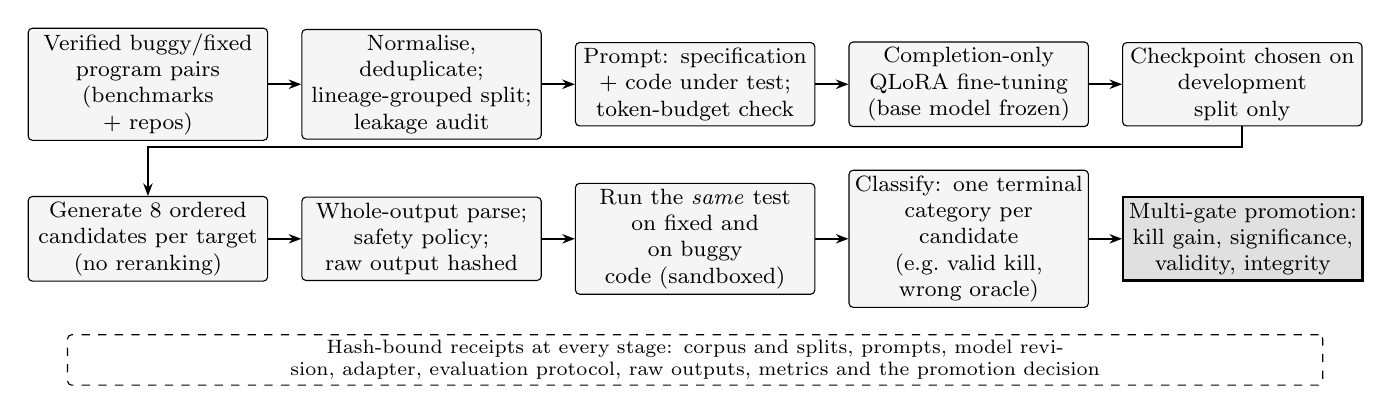
\begin{tikzpicture}[
  font=\footnotesize,
  stage/.style={draw, rounded corners=1.5pt, align=center, minimum height=10.5mm,
                text width=29mm, inner sep=2pt, fill=black!4},
  gate/.style={draw, thick, align=center, minimum height=10.5mm, text width=29mm,
               inner sep=2pt, fill=black!12},
  arr/.style={-{Stealth[length=1.6mm]}, semithick},
  lane/.style={font=\scriptsize\itshape, anchor=west, text=black!70},
  node distance=4.2mm and 4.2mm]

% Row 1: data and training
\node[stage] (pairs) {Verified buggy/fixed\\program pairs\\(benchmarks + repos)};
\node[stage, right=of pairs] (split) {Normalise, deduplicate;\\lineage-grouped split;\\leakage audit};
\node[stage, right=of split] (prompt) {Prompt: specification\\+ code under test;\\token-budget check};
\node[stage, right=of prompt] (sft) {Completion-only\\QLoRA fine-tuning\\(base model frozen)};
\node[stage, right=of sft] (ckpt) {Checkpoint chosen on\\development split only};

% Row 2: evaluation
\node[stage, below=7mm of pairs] (gen) {Generate 8 ordered\\candidates per target\\(no reranking)};
\node[stage, right=of gen] (parse) {Whole-output parse;\\safety policy;\\raw output hashed};
\node[stage, right=of parse] (exec) {Run the \emph{same} test\\on fixed and on buggy\\code (sandboxed)};
\node[stage, right=of exec] (cls) {Classify: one terminal\\category per candidate\\(e.g.\ valid kill, wrong oracle)};
\node[gate, right=of cls] (gate) {Multi-gate promotion:\\kill gain, significance,\\validity, integrity};

\draw[arr] (pairs) -- (split);
\draw[arr] (split) -- (prompt);
\draw[arr] (prompt) -- (sft);
\draw[arr] (sft) -- (ckpt);
\draw[arr] (ckpt.south) -- ++(0,-2.6mm) -| (gen.north);
\draw[arr] (gen) -- (parse);
\draw[arr] (parse) -- (exec);
\draw[arr] (exec) -- (cls);
\draw[arr] (cls) -- (gate);

% Receipts band
\node[draw, dashed, rounded corners=1.5pt, below=5mm of exec, text width=158mm,
      align=center, font=\scriptsize, inner sep=2pt] (rcpt)
      {Hash-bound receipts at every stage: corpus and splits, prompts, model revision,
       adapter, evaluation protocol, raw outputs, metrics and the promotion decision};
\end{tikzpicture}

\caption{Oneiros workflow. Data and training stages (top) produce a checkpoint chosen
only on the development split; evaluation stages (bottom) execute each candidate on
both the fixed and the faulty program, classify it, and apply a multi-gate promotion
rule. Every stage writes a hash-bound receipt.}
\label{fig:workflow}
\end{figure*}

\textbf{Verified program pairs.} Each record pairs a correct (fixed) implementation
with a faulty one. Function-level records are mutants of benchmark solutions, grouped
by mutation family (e.g.\ boundary, arithmetic, comparison). Repository records are
real defects with official reproductions from SWE-bench Verified and BugsInPy. A record
is admitted only if at least one reference-valid, mutation-killing test exists for it
under the current policy.

\textbf{Normalisation and lineage-controlled splitting.} Records are normalised to one
prompt schema and split by semantic group, so all mutants of one original function
fall in the same split. A leakage audit checks for verbatim reference code in prompts
and for lineage links from gold tests, gold patches and oracles.

\textbf{Prompt and target.} The prompt contains the task specification and the code
under test, within fixed token budgets. The supervised target is a verified
mutation-killing test that has already been executed against both versions.

\textbf{Completion-only QLoRA fine-tuning.} The base model is loaded with 4-bit
NormalFloat (NF4) quantization and frozen; low-rank adapters are trained on the
completion tokens only. Checkpoints are selected on the development split; the locked
validation split is read once, after selection, under a decision rule frozen
beforehand.

\textbf{Generation and parsing.} For each target the model emits eight ordered
candidates with no reranking. Each raw output is retained and hashed, and the whole
output is parsed as one test (the \emph{whole-output} protocol; see
Section~\ref{sec:threats}). A safety policy rejects unsafe constructs before execution.

\textbf{Dual execution and classification.} The \emph{same} candidate runs in a
sandbox on the fixed and on the faulty implementation. Each candidate receives exactly
one terminal category, by fixed precedence: \emph{parse failure};
\emph{duplicate} (whitespace-normalised code equal to an earlier candidate for the same
target); \emph{valid kill} (passes on fixed, fails on faulty); \emph{execution
failure} (does not reach its assertions on the fixed code); \emph{non-discriminating
input} (no call behaves differently on the mutant); \emph{discriminating wrong oracle}
(a call behaves differently, but an assertion fails on the correct code); and
\emph{valid non-kill} (correct but too weak to fail on the mutant). A target is
killed at $k$ if any of its first $k$ candidates is a valid kill (\killk{k}).

\textbf{Receipts.} Corpus, splits, model revision, adapter, protocol, source tree,
raw outputs, metrics and decisions are bound by Secure Hash Algorithm (SHA-256)
digests. A full-scale rehearsal of the evaluation path reproduced the recorded
base-model development \killk{8} exactly (0.605166) over 4,336 candidates with zero
missing or mismatched raw-output hashes, which validates the pipeline, not the model.

%=====================================================================================
\section{Dataset and Experimental Setup}

\begin{table}[t]
\centering
\caption{Corpus V4.1: Sources, Split Roles and Training Selection}
\label{tab:data}
\footnotesize
\setlength{\tabcolsep}{3pt}
\begin{tabular}{@{}lr p{0.42\columnwidth}@{}}
\toprule
\multicolumn{3}{@{}l}{\textit{Records by source (8,237; 7,644 function, 593 repository)}}\\
MBPP & 6,384 & synthetic mutants\\
HumanEval & 1,252 & synthetic mutants\\
SWE-bench Verified & 324 & real repository defects\\
BugsInPy & 269 & real repository defects\\
Manually curated & 8 & seeded examples\\
\midrule
\multicolumn{3}{@{}l}{\textit{Splits (records / semantic groups) and role}}\\
Train & 6,052 / 683 & training pool only\\
Development & 594 / 63 & checkpoint selection (542 evaluated)\\
Locked validation & 781 / 82 & read once (757 evaluated)\\
Sealed test & 810 / 94 & consumed by a failed run; no metrics\\
\midrule
\multicolumn{3}{@{}l}{\textit{Fine-tuning selection}}\\
Selected pairs & 2,400 & 2,194 synthetic, 206 repository\\
Pair sources & \multicolumn{2}{p{0.62\columnwidth}}{MBPP 1,776; HumanEval 413; SWE-bench 132; BugsInPy 74; manual 5}\\
Synthetic complexity & \multicolumn{2}{l}{complex 1,317; moderate 610; simple 267}\\
Unique examples & 5,735 & distinct supervised examples\\
Weighted exposures & 6,889 & repetition, not new data; repository share 0.20\\
\midrule
\multicolumn{3}{@{}l}{\textit{Repository-native panel (exploratory)}}\\
Frozen panel & 34 & 25 complex, 7 moderate, 2 simple; 15 repositories\\
Native-executable & 29 & 22 complex, 5 moderate, 2 simple; 14 repositories\\
\bottomrule
\end{tabular}
\end{table}

\textbf{Corpus and roles.} Table~\ref{tab:data} summarises corpus V4.1; its four
splits sum to the 8,237 records. Repository records are excluded from every kill rate
reported in Section~\ref{sec:results}, because they need a native project environment;
only function-mode targets are scored (542 on development, 757 on locked validation).
The leakage audit scanned all 8,237 records: zero verbatim reference leaks, zero
gold-test, gold-patch or oracle lineage failures, and 14 partial-overlap flags, all
manually reviewed.

\textbf{Complexity.} Function tiers come from the abstract syntax tree (AST) of the
faulty function: \emph{complex} if any of cyclomatic complexity $\geq 6$, control
nesting $\geq 3$, logical lines $\geq 24$ or AST nodes $\geq 80$ holds;
\emph{moderate} at $3/2/12/40$; otherwise \emph{simple}. Repository regions use larger
thresholds plus a branch count. Complex functions make up 1,317 of the 2,194 synthetic
training pairs, and 25 of the 34 repository-native targets.

\textbf{Model and training.} The base model is Qwen2.5-Coder-1.5B-Instruct at
immutable Hugging Face revision
\texttt{2e1fd397ee46e1388853d2af2c993145b0f1098a}. The 2,400 selected pairs yield
5,735 unique supervised examples; repository examples are repeated so that they form
20\% of 6,889 weighted exposures, which adds exposure, not new data. Training used
seed 42, LoRA rank 16, $\alpha=32$, dropout 0.05 on the query, key, value and output
projections, NF4 quantization without double quantization, bfloat16 (BF16) compute,
the AdamW optimizer at learning rate $10^{-5}$ with a constant schedule after 25
warm-up steps, gradient clipping at 1.0, batch size 1 with 16-step gradient
accumulation (16 examples per optimizer step), and one epoch of 431 optimizer steps;
A@431 is the final checkpoint. Token budgets were 1,024 (prompt), 1,024 (completion)
and 3,072 (sequence). Software: Python 3.12.14, PyTorch 2.5.1, Transformers 4.48.3 and
PEFT 0.14.0.

\textbf{Frozen evaluation protocol.} Eight candidates per target, temperature 0.7,
top-$p$ 0.9, seed 42, whole-output parsing, the same token budgets, raw outputs
retained, no reranking. Confidence intervals (CIs) for single rates are Wilson
95\%~\cite{wilson1927probable}; paired comparisons use the exact McNemar
test~\cite{mcnemar1947note} over targets and a paired bootstrap (10,000 resamples)
clustered by semantic group.

\textbf{Predeclared promotion rule.} Promotion required all of: (1)~a locked
\killk{8} gain of at least $+3.0$ points, a net gain of at least 15 targets, and
McNemar $p<0.01$; (2)~a reference-validity drop of at most 12 points; (3)~parse and
execution drops of at most 1 point each; (4)~no diversity collapse; and (5)~run
integrity.

%=====================================================================================
\section{Results}
\label{sec:results}

\begin{table}[t]
\centering
\caption{Base vs. Fine-Tuned (A@431). Rates in Percent}
\label{tab:main}
\footnotesize
\setlength{\tabcolsep}{1.8pt}
\begin{tabular}{@{}lrrrr@{}}
\toprule
 & \multicolumn{2}{c}{Development ($n$=542)} & \multicolumn{2}{c}{Locked ($n$=757)}\\
\cmidrule(lr){2-3}\cmidrule(l){4-5}
Metric & Base & A@431 & Base & A@431\\
\midrule
\killk{1} & 23.43 & 34.13 & 23.65 & 23.91\\
\killk{4} & 48.34 & 57.93 & 47.29 & 47.95\\
\killk{8} & \textbf{60.52} & \textbf{69.56} & \textbf{59.45} & \textbf{62.88}\\
Targets killed at 8 & 328 & 377 & 450 & 476\\
\killk{8} Wilson CI & [56.3, 64.5] & [65.6, 73.3] & [55.9, 62.9] & [59.4, 66.2]\\
Parse success & 98.34 & 99.82 & 98.73 & 98.88\\
Execution-valid & 94.86 & 99.31 & 92.83 & 94.22\\
Reference-valid & \textbf{56.55} & \textbf{45.50} & \textbf{45.21} & \textbf{33.34}\\
\midrule
$\Delta$\killk{8} (points) & \multicolumn{2}{c}{$+9.04$} & \multicolumn{2}{c}{$+3.43$}\\
Gained / lost targets & \multicolumn{2}{c}{100 / 51} & \multicolumn{2}{c}{114 / 88}\\
Exact McNemar $p$ & \multicolumn{2}{c}{$8.2\times10^{-5}$\,$^\dagger$} & \multicolumn{2}{c}{0.0783}\\
Clustered CI, $\Delta$\killk{8} & \multicolumn{2}{c}{--} & \multicolumn{2}{c}{[$-4.03$, $+10.88$]}\\
$\Delta$ reference-valid (points) & \multicolumn{2}{c}{$-11.05$} & \multicolumn{2}{c}{$-11.87$}\\
\bottomrule
\multicolumn{5}{@{}p{0.95\columnwidth}@{}}{\scriptsize $^\dagger$The development split
selected the checkpoint, so this value is optimistically biased and is not
generalisation evidence.}
\end{tabular}
\end{table}

\textbf{RQ1 -- mutation killing.} Table~\ref{tab:main} gives the results. On the
development split, A@431 raised \killk{8} from 60.52\% to 69.56\% ($+9.04$ points;
100 targets gained, 51 lost). Because that split chose the checkpoint, this is a
selection statistic. On locked validation, read once, the gain was $+3.43$ points
(59.45\% to 62.88\%; 114 gained, 88 lost, net $+26$). The exact McNemar $p$ was 0.0783,
and the 95\% CI clustered over 78 semantic groups, $[-4.03, +10.88]$, includes zero.
The minimum effect detectable with 80\% power at this cluster count is about 10.7
points. \killk{1} and \killk{4} changed little on locked validation ($+0.26$ and
$+0.66$ points). The development gain therefore transferred only partly, and the
locked gain is not statistically established; this is not evidence that the true
effect is zero.

\textbf{RQ2 -- validity.} Reference validity, the share of candidates that pass on the
correct program, fell by 11.05 points on development and by 11.87 points on locked
validation (45.21\% to 33.34\%; clustered CI $[-20.09, -3.26]$). Targets with at least
one reference-valid candidate fell from 675 to 566 of 757. Parse and execution rates
did not fall, so the regression is in test \emph{content}, not syntax or runnability.

\begin{table}[t]
\centering
\caption{Terminal Categories on Locked Validation (6,056 Candidates per Arm)}
\label{tab:taxonomy}
\footnotesize
\setlength{\tabcolsep}{4pt}
\begin{tabular}{@{}lrrrr@{}}
\toprule
 & \multicolumn{2}{c}{Base} & \multicolumn{2}{c}{A@431}\\
\cmidrule(lr){2-3}\cmidrule(l){4-5}
Category & Count & \% & Count & \%\\
\midrule
Valid kill & 975 & 16.10 & 1,105 & 18.25\\
Discriminating wrong oracle & 1,863 & 30.76 & \textbf{2,736} & \textbf{45.18}\\
Non-discriminating input & 1,226 & 20.24 & 1,127 & 18.61\\
Valid non-kill (weak oracle) & 497 & 8.21 & 1 & 0.02\\
Duplicate & 1,118 & 18.46 & 817 & 13.49\\
Execution failure & 300 & 4.95 & 202 & 3.34\\
Parse failure & 77 & 1.27 & 68 & 1.12\\
\bottomrule
\end{tabular}
\end{table}

\begin{table}[t]
\centering
\caption{Stage Rates on Locked Validation (Percent; $\Delta$ with 95\% CI Clustered over 78 Semantic Groups)}
\label{tab:stages}
\footnotesize
\setlength{\tabcolsep}{2.5pt}
\begin{tabular}{@{}lrrr@{}}
\toprule
Stage & Base & A@431 & $\Delta$ [95\% CI]\\
\midrule
Discriminating $\mid$ executed & 73.37 & 77.74 & $+4.37$ [1.94, 6.94]\\
Correct oracle $\mid$ discriminating & 47.03 & 33.18 & $-13.85$ [$-22.52$, $-4.80$]\\
\quad same, equality asserts only$^\ast$ & 37.39 & 33.14 & $-4.25$ [$-11.09$, 2.67]\\
Equality-form assertions & 72.47 & 99.50 & $+27.03$ [18.56, 35.62]\\
Kill $\mid$ reference-valid & 50.95 & 72.71 & $+21.76$ [11.73, 31.82]\\
\bottomrule
\multicolumn{4}{@{}p{0.95\columnwidth}@{}}{\scriptsize $^\ast$Form-stratified metric
added after the first analysis; reported alongside, not instead of, the predeclared
unstratified row.}
\end{tabular}
\end{table}

\textbf{RQ3 -- failure categories.} Table~\ref{tab:taxonomy} shows where the
candidates went. Fine-tuning added 130 valid kills but 873 discriminating wrong
oracles, and nearly eliminated weak (valid non-kill) tests. Table~\ref{tab:stages}
decomposes the pipeline. The fine-tuned model chose discriminating inputs more often
($+4.37$ points) and, once its test was valid, killed far more often ($+21.76$). But
given a discriminating input, its assertion held on the correct program much less
often ($-13.85$). The model also shifted almost all assertions to exact equality
(72.47\% to 99.50\%). Restricted to equality assertions, the change in oracle
correctness was $-4.25$ points with an interval that includes zero. The more cautious
reading is that fine-tuning changed \emph{input choice and assertion form} but did not
demonstrate an improvement in predicting the correct value: sharper assertions turn
uncertain value predictions into both more kills and more wrong oracles. At the target
level, 69 targets gained and 150 lost a valid discriminating candidate.

\textbf{Promotion decision.} Criterion~1 failed on significance ($p=0.0783$ against
$p<0.01$), although its gain ($\geq +3.0$) and net ($\geq 15$) parts passed. Criterion~2
\emph{passed}: the 11.87-point validity drop was inside the predeclared 12-point
allowance. Criterion~5 failed because of a harness defect in the integrity gate: a
late implementation change incorrectly treated the arm-specific adapter hash as a
cross-arm invariant in the run-contract comparison, so a fine-tuned arm could never
match the base arm. The adapter itself was not defective, and the defect did not turn
the non-significant locked result into a positive one: the base model was already
retained because the predeclared significance gate failed. We recorded the defect as a
failure rather than reinterpreting the criterion.

\textbf{RQ4 -- repository-native evidence.} The frozen pool contained 70 repositories:
52 entered the scan stage (17 were excluded at screening and 1 was unavailable), and
804 candidate fixes were evaluated. The acquisition gate recorded 114 admissions;
removing one within-set duplicate leaves 113 unique functions from 31 repositories. Of
these, 85 had an authenticated, non-overlapping regression test, 51 qualified
natively, 46 requalified in three of three runs, 45 reached the target on both
revisions, and 36 passed prompt-leakage and token-fit checks; 34 targets from 15
repositories were frozen as the panel. Twenty-nine targets from 14 repositories are
executable under the sandbox policy; 5 were excluded before any generation because the
policy blocks native-library loading. These are environment exclusions, not model
failures. The predeclared minimum for a confirmatory panel was 80 targets from 10
repositories, so the panel is exploratory. For the 29 native-executable targets, a
planning analysis that borrowed the locked comparison's discordance rate (0.267)
estimated that a difference of about 26.3 percentage points would be needed for 80\%
power at $\alpha=0.05$; at the predeclared $\alpha=0.01$, no effect up to the
26.7-point maximum allowed by that discordance reached 80\% power. A three-arm
generation plan (base, A@431 and a relearning checkpoint) with a frozen analysis
passed all 17 preflight checks, but \textbf{no repository-native generation has yet
been run}, and no repository-native result is reported.

%=====================================================================================
\section{Discussion}

\textbf{Input selection and oracle prediction are separate skills.} A test must both
reach a state where the fault is visible and predict the correct output there. Our
measurements separate the two. Fine-tuning improved discriminating-input selection but
did not demonstrate an improvement in expected-value prediction. Because a kill
requires only that the faulty program disagrees with the asserted value, a model that
asserts \emph{some} value more forcefully on a better input can raise \killk{8} while
more of its tests are wrong for the correct program. \killk{8} can rise while semantic
validity falls.

\textbf{Why the checkpoint was not promoted.} The locked gain was positive but not
statistically established, and the development gain was optimistic because of
selection. A rule based on \killk{8} alone, especially on the selection split, would
have promoted a model that produced 873 more wrong-oracle candidates on the locked
split.

\textbf{Lessons for promotion rules.} Our frozen rule allowed a validity drop of up to
12 points, and the observed drop (11.87) passed. In hindsight that allowance was too
loose: a promotion gate should treat validity and wrong-oracle growth as
\emph{blocking}, not as tolerances around a kill-rate gain.

\textbf{Implications.} Studies that report mutation score or pass rate for
LLM-generated tests should also report how many candidates fail on the correct
program, and should select checkpoints on one split and report on another.

\textbf{Implementation experience.} In our work, aggregate \killk{8} alone concealed
the failure modes that mattered. Only because complete generations were retained and
every candidate was executed against both program versions could we see that
fine-tuning increased valid kills (975 to 1,105) while increasing discriminating
wrong-oracle failures far more (1,863 to 2,736). This finding led us to candidate-level
failure classification, to the recommendation that validity act as a blocking gate,
and to oracle-focused training as the next line of work. It concerns the
function-level splits only; repository-native behaviour has not yet been measured.

%=====================================================================================
\section{Threats to Validity and Limitations}
\label{sec:threats}

\textbf{Scale and data.} One 1.5B model and one training seed were evaluated. Training
data are dominated by MBPP and HumanEval mutants; real repository defects form a
small share. Results may not hold for larger models, other languages or other fault
types.

\textbf{Pretraining contamination.} The base model may have encountered HumanEval or
MBPP tasks during pretraining. The paired base-versus-adapter comparison controls
shared exposure between arms but does not remove benchmark memorization as a threat to
the absolute performance rates. Our leakage audit covers the project's own splits, not
the model's pretraining data.

\textbf{Statistical power.} With 757 targets in 78 semantic groups, the locked study
could reliably detect only gains of about 10.7 points; a non-significant result is not
evidence of no effect. The locked split has now been used and therefore cannot provide
a second independent confirmation; retained outputs may be rescored only for declared
diagnostic analyses.

\textbf{Sealed test.} The single authorised sealed-test run failed during record
admission, before any generation. It produced no candidates and no metrics, and the
split is consumed. No final-test result exists for Oneiros.

\textbf{Evaluator defects found and corrected.} An earlier parser scored only the first
\texttt{assert} line of each output; the whole-output protocol used here replaced it,
and all results in this paper use the corrected protocol. An earlier Atheris baseline
was not coverage-instrumented and passed aliased arguments to reference and mutant; it
was corrected, but its figures were measured under the earlier test protocol, so we do
not compare Oneiros with Atheris here. The integrity-gate defect is described in
Section~\ref{sec:results}.

\textbf{Measurement choices.} One terminal category per candidate depends on a fixed
precedence order. The form-stratified oracle metric was added after the first look.
Some HumanEval prompts state an input--output example that kills the mutant, which
inflates HumanEval kill rates. All execution depends on the sandbox policy, which also
excluded 5 repository targets.

\textbf{Repository-native evaluation} remains underpowered and unexecuted.

%=====================================================================================
\section{Conclusion and Future Work}

Fine-tuning a small code model on verified mutation-killing tests raised development
\killk{8} by 9.04 points, but on a locked split the gain was 3.43 points and not
statistically significant, while reference validity fell by 11.87 points. The failure
taxonomy locates the cause: better discriminating-input selection and a shift to
exact-equality assertions, without demonstrated improvement in expected-value
prediction. Oneiros's main contribution is therefore the evaluation and promotion
methodology that caught this, not a better model.

Next steps are to: treat input selection and oracle prediction as separate learning
targets; make validity and wrong-oracle growth blocking promotion gates; build more
unique, execution-verified repository examples and keep replay data during
fine-tuning; complete a sufficiently powered repository-native evaluation on a new,
independently built held-out set; and compare against corrected baselines on identical
eligible subsets.

\section*{Acknowledgment}
\ifanonymous\else
The authors thank Dr.~Priyanka~H for guidance and feedback.
\fi
\ifaidisclosure
Anthropic Claude (Claude Code) assisted in preparing the initial drafts of the
Abstract, Nomenclature, Sections I--VIII, Tables I--IV, Fig.~1 and the reference list
from author-supplied experiment records.
\fi

\balance
\bibliographystyle{IEEEtran}
\bibliography{references}

\end{document}
